\chapter{Introducción}
Si el universo tuvo un principio, como el \textit{Big Bang}, procedente de esa ``explosión'' la distribución de materia y energía habría sido muy irregular. Enormemente difusa. El tiempo y el espacio habrían estado curvados, retorcidos, deformados.

Pero cuando miramos al universo hoy, no vemos nada de eso. La distribución de materia y energía es casi uniforme en el universo, y el propio espacio es extremadamente plano, obedeciendo a las leyes de la geometría más sencilla. Así que, ¿cómo llegamos desde ese salvaje estado inicial hasta el presente? Ahí es donde nació la idea de inflación.

El concepto que introdujo la inflación es que, después del \textit{Big Bang}, quizás hubo un periodo de expansión muy rápida y acelerada, expandiendo el universo tan rápido que lo convertiría en algo aplanado y uniforme, y la distribución de materia y energía habría sido también uniformada de esta manera.

La teoría inflacionaria~\cite{albrecht1982cosmology,guth1981inflationary,linde1982new}, uno de los ejes centrales de la Cosmología moderna, fue introducida por Alan Guth ---entre otros--- en 1981 para resolver una serie de problemas~\cite{peebles1993principles} que estaban presentes en el marco teórico de la Cosmología de la época: el \textit{Hot Big Bang}. En la~\autoref{fig::guth} se muestra una parte de sus notas originales.
\begin{figure}[t]
    \centering
    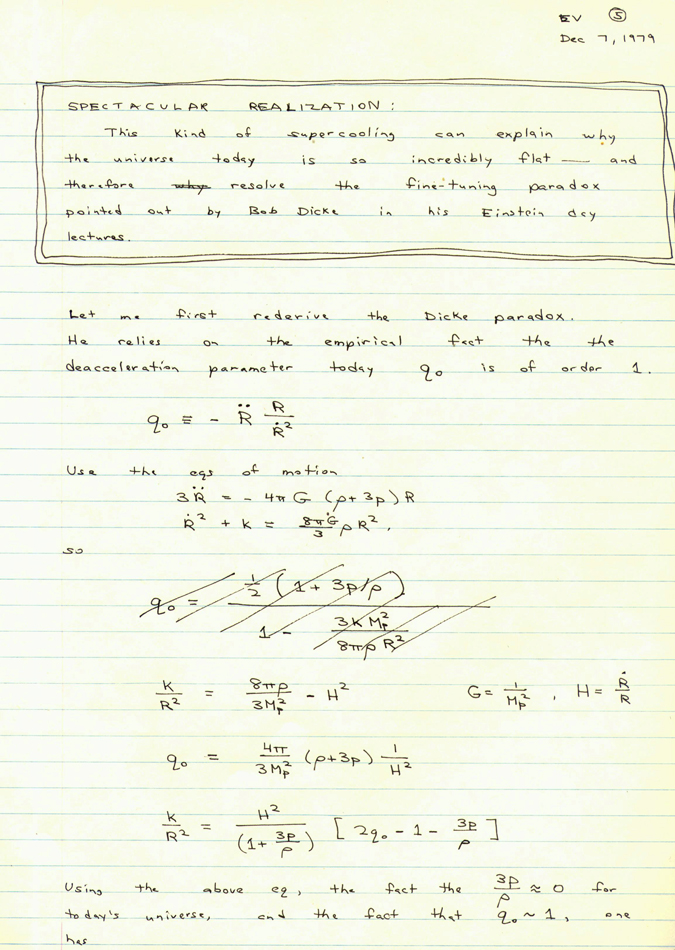
\includegraphics[scale=1.06]{img/AlanGuth.jpg}
    \caption{Cuaderno con la idea original de Guth}
    \label{fig::guth}
\end{figure}

Una de las asombrosas características de la inflación es que encierra un mecanismo para producir las fluctuaciones de densidad primordiales. Estas pequeñas fluctuaciones cuánticas son estiradas por la expansión inflacionaria y se convierten en las semillas para la formación de la estructura a gran escala del universo~\cite{Mukhanov1981,bardeen1983spontaneous,hawking1982development,starobinsky1982dynamics,guth1985quantum}. Dichas fluctuaciones se describen mediante campos aleatorios, que son la generalización de las variables aleatorias a cantidades que toman valores diferentes en distintos puntos del espacio y/o del tiempo. La estadística de los campos aleatorios está codificada en el espectro de potencias \(P(k)\), donde \(k\) es el módulo del vector de onda comóvil.
\newpage
Sin embargo, si se proporciona un \(P(k)\), no es muy sencillo visualizar cómo sería el correspondiente mapa espacial de fluctuaciones, lo que dificulta la intuición de lo que significa un espectro de potencia concreto. En este trabajo, mediante el uso del lenguaje de programación \textit{Python}, se generarán y representarán realizaciones de distintos campos aleatorios gaussianos de densidad.
\clearpage
\section{El universo homogéneo e isótropo}\label{sec::homogeneo}
La cosmología física necesita un marco teórico que permita explicar los datos observacionales. En ausencia de dicho marco, ni siquiera las propiedades observables más básicas de las galaxias, como el desplazamiento al rojo, el brillo o tamaño aparentes, podrían interpretarse correctamente. El actual marco teórico aceptado por la mayoría de los astrónomos es el ``modelo de concordancia'' ---dentro de la teoría del \textit{Big Bang}--- que es un modelo basado en la métrica Friedmann-Lemaître-Robertson-Walker (FLRW). Estos modelos están basados en la suposición de que el universo se rige por la relatividad general y es esencialmente homogéneo e isótropo, si se suaviza en escalas suficientemente grandes.
\subsection{Principio cosmológico}
La cosmología moderna se apoya en dos principios fundamentales: en primer lugar, la interacción dominante en escalas cosmológicas es la gravedad, y segundo, el principio cosmológico es una buena aproximación del universo. El principio cosmológico afirma que el universo, suavizado en escalas suficientemente grandes, es esencialmente homogéneo e isótropo. La homogeneidad tiene el significado intuitivo de que en un momento dado, el universo se ve igual en todas partes, e isotropía se refiere al hecho de que para cualquier observador que se mueve con la materia local, el universo se ve (localmente) igual en todas las direcciones.
\subsection{El \textit{Hot Big Bang}}
La teoría estándar del \textit{Hot Big Bang} es considerablemente exitosa, superando algunas pruebas clave de observación: expansión del universo, la existencia y espectro del \textit{Cosmic Microwave Background} (CMB), las abundancias de elementos ligeros en el universo (nucleosíntesis)~\cite{gamow1946expanding,alpher1948evolution,alpher1953physical}, entre otras~\cite{liddle1998introduction}.

El universo se está expandiendo~\cite{hubble1929relation}. Era entonces más denso y caliente en el pasado. Las partículas colisionaban frecuentemente y el universo estaba en un estado de equilibrio térmico con una temperatura \(T\). Ajustando la constante de Boltzmann a la unidad \(k_B=1\), se mide la temperatura en unidades de energía. De este modo, midiendo las energías en electronvoltios:
\begin{equation}
    \mathrm{eV}\approx 1.6\times 10^{-19}\,\mathrm{J}\approx 1.2\times 10^{4}\,\mathrm{K}.
\end{equation}
La relación entre la temperatura del universo temprano y su edad es~\cite{baumann2022cosmology}
\begin{equation}
    \frac{T}{1\,\mathrm{MeV}}\simeq \left(\frac{t}{1\,\mathrm{s}}\right)^{-1/2}.
\end{equation}
Un segundo después del \textit{Big Bang} la temperatura del universo era de unos \(10^{11}\) K (o 1 MeV). Como aún había pasado poco tiempo en el universo temprano, la cadencia de las reacciones era extremadamente alta, así que pasaron muchas cosas en un corto periodo de tiempo (véase~\autoref{tab::eventos}).
    {\renewcommand{\arraystretch}{1.1}
        \begin{table}[t]
            \centering
            \caption{Eventos clave en la historia del universo}
            \label{tab::eventos}
            \begin{tabular}{lrrr}
                \toprule
                \multicolumn{1}{c}{\textbf{Evento}}               & \textbf{temperatura}                                              & \textbf{energía}                                                  & \textbf{tiempo}                                                   \\ \midrule
                \rowcolor{migris!50}
                {\color[HTML]{FFFFFF} Inflación}                  & {\color[HTML]{FFFFFF} \(<10^{28}\) K}                             & {\color[HTML]{FFFFFF} \(<10^{16}\) GeV}                           & {\color[HTML]{FFFFFF} \(>10^{-34}\) s}                            \\
                Desacoplamiento materia oscura                    & \multicolumn{1}{c}{?}                                             & \multicolumn{1}{c}{?}                                             & \multicolumn{1}{c}{?}                                             \\
                \rowcolor{migris!50}
                {\color[HTML]{FFFFFF} Formación de bariones}      & \multicolumn{1}{c}{\cellcolor{migris!50}{\color[HTML]{FFFFFF} ?}} & \multicolumn{1}{c}{\cellcolor{migris!50}{\color[HTML]{FFFFFF} ?}} & \multicolumn{1}{c}{\cellcolor{migris!50}{\color[HTML]{FFFFFF} ?}} \\
                Transición de fase electrodébil                   & \(10^{15}\) K                                                     & \(100\) GeV                                                       & \(10^{-11}\) s                                                    \\
                \rowcolor{migris!50}
                {\color[HTML]{FFFFFF} Formación de hadrones}      & {\color[HTML]{FFFFFF} \(10^{12}\) K}                              & {\color[HTML]{FFFFFF} \(150\) MeV}                                & {\color[HTML]{FFFFFF} \(10^{-5}\) s}                              \\
                Desacoplamiento de neutrinos                      & \(10^{10}\) K                                                     & \(1\) MeV                                                         & \(1\) s                                                           \\
                \rowcolor{migris!50}
                {\color[HTML]{FFFFFF} Formación de núcleos}       & {\color[HTML]{FFFFFF} \(10^{9}\) K}                               & {\color[HTML]{FFFFFF} \(100\) KeV}                                & {\color[HTML]{FFFFFF} \(200\) s}                                  \\
                Formación de átomos                               & \(3400\) K                                                        & \(0.30\) eV                                                       & \(250\,000\) a                                                    \\
                \rowcolor{migris!50}
                {\color[HTML]{FFFFFF} Desacoplamiento de fotones} & {\color[HTML]{FFFFFF} \(2900\) K}                                 & {\color[HTML]{FFFFFF} \(0.25\) eV}                                & {\color[HTML]{FFFFFF} \(380\,000\) a}                             \\
                Primeras estrellas                                & \(50\) K                                                          & \(4\) meV                                                         & \(100\) Ma                                                        \\
                \rowcolor{migris!50}
                {\color[HTML]{FFFFFF} Primeras galaxias}          & {\color[HTML]{FFFFFF} \(20\) K}                                   & {\color[HTML]{FFFFFF} \(1.7\) meV}                                & {\color[HTML]{FFFFFF} \(1\) Ga}                                   \\
                Sistema solar                                     & \(3.8\) K                                                         & \(0.33\) meV                                                      & \(9\) Ga                                                          \\
                \rowcolor{migris!50}
                {\color[HTML]{FFFFFF} Escritura de este TFG}      & {\color[HTML]{FFFFFF} \(2.7\) K}                                  & {\color[HTML]{FFFFFF} \(0.23\) meV}                               & {\color[HTML]{FFFFFF} \(13.8\) Ga}                                \\ \bottomrule
            \end{tabular}
        \end{table}}

Un acontecimiento importante en la historia del universo primitivo es la formación de los primeros átomos y el consecuente desacoplamiento de los fotones (véase~\autoref{fig::decouple}). Ocurrió 380 000 años después del \textit{Big Bang} y se le conoce por \textbf{recombinación}. En este punto, la temperatura era lo suficientemente baja ---debajo de 0.3 eV--- para que se formaran átomos de hidrógeno mediante la reacción \(\mathrm{e^{-}}+\mathrm{p^+}\rightarrow \mathrm{H}+\gamma\). Alrededor de 0.25 eV, los fotones se desacoplaron de la materia y el universo se torna transparente. Estos fotones todavía se ven hoy en día como un resplandor del \textit{Big Bang}. Estirada por 13 800 millones de años de expansión cósmica, la primera luz del universo se observa hoy como una débil radiación de microondas, el CMB~\cite{penzias1965measurement}.
\begin{figure}
    \centering
    \def\svgwidth{0.9\textwidth}
    \input{svg/cmb.pdf_tex}
    \caption[Representación de la recombinación de protones y electrones]{Representación de la recombinación de protones y electrones en átomos de hidrógeno neutros y el correspondiente desacoplamiento de los fotones}
    \label{fig::decouple}
\end{figure}

Una característica destacable de las correlaciones observadas en el CMB es que abarcan escalas mayores que la distancia recorrida por la luz entre el inicio del \textit{Hot Big Bang} y el momento en que se creó el CMB. Esto entra en conflicto con la causalidad, a menos que las correlaciones se generaran antes del \textit{Hot Big Bang}. De hecho, cada vez hay más pruebas de que el \textit{Big Bang} no fue el comienzo del tiempo, sino que las fluctuaciones de densidad primordiales se produjeron durante un periodo anterior de expansión acelerada llamado inflación.

Aun así, surgen dilemas en esta teoría ya que se limita a aquellas épocas en las que el universo es lo suficientemente frío para que los procesos físicos fundamentales que subyacen estén bien consolidados y comprendidos a través de la experiencia en la Tierra; no aborda el estado del universo en momentos anteriores, más calientes. Estas cuestiones cruciales sin respuesta en el \textit{Hot Big Bang} ---precursoras en la introducción de la inflación--- son el problema de la \textbf{planitud}, el problema del \textbf{horizonte} y la existencia de \textbf{monopolos magnéticos}. Tanto la primera como la segunda son el objeto de estudio de este texto al estar relacionadas con las condiciones iniciales del universo, que tuvieron que ser muy especiales y finamente ajustadas para dar lugar a lo que se observa hoy día. La última, la existencia de monopolos magnéticos y otras partículas que hoy no se observan pero deberían estar ahí~\cite{liddle1998introduction}, también queda resuelta con inflación pero no se dirá más sobre ella en este escrito.

Para especificar las condiciones iniciales del \textit{Hot Big Bang}, se definen las posiciones y velocidades de todas las partículas en un intervalo de tiempo inicial, o aproximando al universo como un fluido la presión y densidad. Las leyes de la gravedad se utilizan entonces para hacer evolucionar el sistema en el tiempo. En la teoría estándar del \textit{Big Bang} se supone la distribución de materia como homogénea e isotrópica~\cite{baumann2022cosmology}. Pero, ¿cómo se explica esta uniformidad del universo temprano? Incluso es algo que contrasta con la imagen proyectada por la teoría del \textit{Big Bang} donde la mayor parte del universo parece no haber estado en contacto causal y no hay motivo dinámico para que estas regiones causalmente no conectadas tengan tales propiedades físicas similares que se suponen. Este problema de la homogeneidad se conoce como el problema del \textbf{horizonte}.

\begin{figure}[t]
    \centering
    \def\svgwidth{0.75\textwidth}
    \input{svg/horizonproblem.pdf_tex}
    \caption[Ilustración del problema del horizonte]{Ilustración del problema del horizonte en el modelo convencional del \textit{Big Bang}. Todos los eventos que observamos actualmente están en nuestro cono de luz pasado. La intersección de nuestro cono de luz del pasado con la franja espacial en el momento de la recombinación es la superficie de última dispersión. Los puntos que están separados por más de 2° en el cielo parecen no haber estado nunca haber estado en contacto causal, ya que sus conos de luz pasados no se solapan. Notar que la singularidad del \textit{Big Bang} es un momento en el tiempo y no un punto en el espacio.}
    \label{fig::horizonproblem}
\end{figure}
Para visualizar el primer problema, considérense dos direcciones opuestas en el cielo. Los fotones del CMB que recibimos de dichas direcciones fueron emitidos en los puntos etiquetados como \(q\) y \(p\) en la~\autoref{fig::horizonproblem}. Se observa que los fotones fueron liberados lo suficientemente cerca de la singularidad del \textit{Big Bang} para que los conos de luz del pasado de \(q\) y \(p\) no se superpongan. Como ningún punto se encuentra dentro de los horizontes de \(q\) y \(p\), tenemos el siguiente enigma: ¿Cómo ``saben'' los fotones procedentes de estos dos puntos que deben estar a la misma temperatura? Simplemente no hubo tiempo suficiente para que las diferencias en las temperaturas iniciales se eliminaran mediante transferencia de calor. Lo mismo se aplica para cualesquiera dos puntos en el CMB que estén separados por más de 2°~\cite{baumann2022cosmology}.

\begin{figure}
    \centering
    \def\svgwidth{0.72\textwidth}
    \input{svg/horizonproblemsol.pdf_tex}
    \caption[Solución inflacionaria al problema del horizonte]{Solución inflacionaria al problema del horizonte. La singularidad del \textit{Big Bang} estándar se sustituye por la superficie de recalentamiento. En lugar de marcar el comienzo del tiempo, ahora corresponde a la transición de la inflación a la evolución clásica del \textit{Big Bang}. Todos los puntos del CMB tienen conos de luz pasados que se superponen y, por tanto, se originan en una región del espacio conectada causalmente.}
    \label{fig::horizonproblemsol}
\end{figure}
En teorías inflacionarias la singularidad de la~\autoref{fig::horizonproblem} no es la singularidad inicial, sino la transición entre inflación y el \textit{Hot Big Bang}. Notar que el tiempo \(t=0\) ahora se traslada a un momento previo. La física sigue manteniendo el tiempo entre la singularidad y recombinación en \(380\,000\) años, pero los conos de luz se estiran drásticamente por la expansión inflacionaria permitiendo que estos se superpongan antes del fin de inflación. Esto es representado esquemáticamente en la~\autoref{fig::horizonproblemsol}.

Para que el universo siga siendo homogéneo en tiempos posteriores, las velocidades iniciales deben tomar valores muy precisos. Si las velocidades iniciales son ligeramente demasiado pequeñas, el universo vuelve a colapsar en una fracción de segundo. Si son demasiado grandes, el universo se expande demasiado rápido y se queda casi vacío. El ajuste de las velocidades iniciales se hace aún más drástico si se considera en combinación con el problema del horizonte, ya que las velocidades de las partículas deben ajustarse a través de regiones del espacio causalmente desconectadas. Este ajuste preciso en la condición inicial de velocidad es lo que se conoce como el problema de la \textbf{planitud} y se plantea comúnmente como por qué la curvatura espacial del universo es tan pequeña, cuya relación con las velocidades viene dada por la suma de la energía cinética y potencial en una determinada región~\cite{baumann2022cosmology}.

Los problemas de causalidad descritos arriba sugieren que hubo una fase antes del \textit{Hot Big Bang}, durante la cual la homogeneidad del universo y sus correspondientes fluctuaciones fueron generadas. Un periodo de expansión acelerada es suficiente para resolverlos. Pero es necesario un escenario viable para dirigir tal expansión. Los campos escalares son la receta a seguir.
\section{Inflación}
Sabemos que para obtener una expansión acelerada, la presión efectiva debe ser negativa~\cite{dodelson2020modern}. Inflación, aparentemente, fue dirigida por una forma de energía cuya presión \(\mathcal{P}<0\). La presión negativa no es algo familiar para los físicos. Así, sea lo que sea que conduce inflación, no es materia ordinaria o radiación. Tampoco puede ser una constante cosmológica: en este caso, el universo estaría en un estado de rápida inflación perpetuo, mientras que necesitamos que el periodo inflacionario termine y exista una transición de la fase dominada por radiación a la fase dominada por materia, ambas conocidas.
\newpage
La forma más simple de generar tal época transitoria de expansión acelerada es mediante la energía potencial de un campo escalar. En física de partículas, se utilizan los campos escalares para representar partículas de espín cero. Se transforman como un escalar (es decir, no cambian) bajo transformaciones de coordenadas. En un universo homogéneo, un campo escalar será función del tiempo únicamente. Notar que no hay campo escalar conocido que pueda regir inflación. Aunque conocemos un campo escalar en la naturaleza, el campo de Higgs, usarlo para dirigir inflación resulta ser complicado. Sus propiedades e interacciones están lo suficientemente restringidas, por ahora, para que sepamos que no puede servir como fuente de la inflación. No obstante, hay que tener en cuenta que puede ser cierto que la idea de la inflación sea correcta, pero esté impulsada por algo distinto a un campo escalar.
\subsection{Dinámica del campo escalar}
Se toman como punto de partida las expresiones de la densidad de energía y presión efectivas de un campo escalar \(\phi\left(t,\symbf{x}\right)\) que llamaremos \textbf{inflatón}. Como se indica en la notación, el valor del campo depende del tiempo \(t\) y de la posición \(\symbf{x}\). Asociado a cada valor del campo hay una densidad de energía potencial \(V(\phi)\). Cuando el campo es dinámico (cambia con el tiempo) entonces también incluye una densidad de energía cinética \(\frac{1}{2}\dot{\phi}^2\). Si la energía asociada al campo escalar domina el universo, entonces sirve como fuente de la evolución de este en el modelo FLRW~\cite{baumann2022cosmology}, donde se tiene al mismo ocupado por un fluido perfecto. Dichas expresiones de la densidad de energía y presión, se obtienen por comparación del tensor energía-momento (ecuaciones relatividad general de Einstein) del campo escalar con el de un fluido perfecto, y son
\begin{subequations}
    \begin{align}
        \rho_\phi&=\frac{1}{2}\dot{\phi}^2+V(\phi)\label{eq::rho}\\
        \mathcal{P}_\phi&=\frac{1}{2}\dot{\phi}^2-V(\phi),
    \end{align}
    \label{eq::eqscampo}
\end{subequations}
respectivamente, donde \(\dot{\phi}\) indica derivada temporal.

En lo sucesivo son utilizadas las unidades naturales, esto es, \(c=\hbar=1\). Definimos la ecuación de estado de un fluido perfecto con el número adimensional \(\mathscr{w}\):
\begin{equation}
    \mathscr{w}\equiv\frac{\mathcal{P}_\phi}{\rho_\phi}.
\end{equation}
El universo está acelerando solo si es gobernado por uno o varios componentes energéticos con ecuaciones de estado \(\mathscr{w}_i<-1/3\)~\cite{knobel2012introduction}. Así que durante inflación se ha de cumplir esta condición.

En el marco FLRW, el campo escalar es homogéneo y por tanto, solo depende del tiempo, esto es, \(\phi\left(t,\symbf{x}\right)\rightarrow\phi(t)\). Este obedece la ecuación de movimiento
\begin{equation}
    \ddot{\phi}+3H\dot{\phi}+V'(\phi)=0,\label{eq::eqmovcampo}
\end{equation}
donde \(V'(\phi)=\mathrm{d}V/\mathrm{d}\phi\) y
\begin{equation}
    H=H(t)\equiv \frac{1}{a}\frac{\mathrm{d}a}{\mathrm{d}t}
\end{equation}
es el parámetro de Hubble, donde \(a(t)\) es el factor de escala (cantidad adimensional) del universo, el cual cuantiza el tamaño físico de este. La forma de \(a(t)\) depende de las propiedades del material dentro del universo~\cite{liddle1998introduction}. El término \(\dot{\phi}^2/2\) en~\ref{eq::eqscampo} es como la ``energía cinética'' del campo y \(3H\dot{\phi}\) en~\ref{eq::eqmovcampo} viene de la expansión del universo y actúa como una fricción. Con las expresiones en~\ref{eq::eqscampo}, la ecuación de estado del campo escalar es
\begin{equation}
    \mathscr{w}(t)=\frac{\frac{1}{2}\dot{\phi}^2-V(\phi)}{\frac{1}{2}\dot{\phi}^2+V(\phi)}\label{eq::estado}
\end{equation}
con los límites \(-1\leq\mathscr{w}(t)\leq 1\). La ecuación de arriba es generalmente dependiente del tiempo. No obstante, si \(\dot{\phi}^2<4V(\phi)\) entonces \(\mathscr{w} < -1/3\) y la condición para inflación es satisfecha. Más aún, si \(\dot{\phi}^2 \ll V(\phi)\), entonces la ecuación de estado se torna \(\mathscr{w}\simeq -1\) y es constante. La expansión asociada del universo es, en este último caso, exponencial con \(H\) y \(\phi\) siendo prácticamente constantes~\cite{knobel2012introduction}.
\subsection{Inflación \textit{Slow-roll}}
Hasta ahora, la forma del potencial \(V(\phi)\) está indeterminada y hay bastantes escenarios de inflación posibles en la literatura, véase~\cite{liddle2000cosmological}. Sin embargo, las predicciones de los modelos más simples de inflación son bastante robustas y de este modo no es necesario especificar todos los detalles siempre y cuando se cumplan ciertas características. El escenario más popular y simple de inflación supone un campo escalar ``rodando lentamente'' (de aquí en adelante se usará el anglicismo \textit{slow-roll} para referirnos a este tipo de escenarios) hacia su estado fundamental~\cite{linde1982new,albrecht1982cosmology}. La energía potencial de un campo escalar \textit{slow-roll} es muy cercana a constante (si el potencial no es muy pronunciado) por lo que rápidamente llega a dominar sobre la energía cinética (y la energía de todas las demás partículas). Un ejemplo es mostrado en la~\autoref{fig::potential}; inflación acaba una vez el campo haya llegado al mínimo del potencial, donde oscilará y decaerá a partículas más ligeras ---eventualmente a aquellas del modelo estándar de partículas--- en un proceso llamado \textbf{recalentamiento} (del que no conocemos los detalles, pero sabemos de varios mecanismos físicos para conseguirlo), siguiendo a este la escena del \textit{Big Bang} que fue discutida en la sección anterior. En ese momento, el campo ya no rueda lentamente, sino que tiene una energía cinética importante, por lo que oscila en torno al mínimo. Entonces, la ecuación de estado~\ref{eq::estado} ya no está cerca de -1, sino cerca de cero, por lo que el universo ha pasado a una época de expansión desacelerada. Entonces, al final, \(\phi\) decae en partículas más ligeras. Con el tiempo, quizá tras una larga cadena de desintegraciones, el resultado es un universo casi completamente homogéneo, dominado por la radiación.
\begin{figure}[t]
    \centering
    \def\svgwidth{0.65\textwidth}
    \input{svg/potential.pdf_tex}
    \caption[Ejemplo de un potencial \textit{slow-roll}]{Ejemplo de un potencial \textit{slow-roll}. Inflación ocurre en la parte sombreada.}
    \label{fig::potential}
\end{figure}
\newpage
Estos modelos contienen un solo campo escalar \(\phi\) (inflatón) y resolver la ecuación de movimiento~\ref{eq::eqmovcampo} se vuelve accesible si hacemos la aproximación \textit{slow-roll} donde el término \(\ddot{\phi}\) es despreciable. La motivación física aquí es que interesa más un comportamiento de expansión, así el potencial domina en la densidad de energía~\cite{peacock1998cosmological}. La condición es
\begin{equation}
    \frac{\dot{\phi}^2}{2}\ll V(\phi);
\end{equation}
diferenciando se obtiene
\begin{equation}
    \ddot{\phi}\ll V'(\phi),
\end{equation}
tal y como se buscaba. De este modo, se tiene una simple ecuación \textit{slow-roll} para campos homogéneos:
\begin{equation}
    3H\dot{\phi}=-V'(\phi).
\end{equation}
Combinando la ecuación anterior con la ecuación de Friedmann~\cite{friedmann1922125}, usando las unidades naturales,
\begin{equation}
    H^2=\frac{8\pi G}{3}\left(\frac{\dot{\phi}^2}{2}+V(\phi)\right)\simeq \frac{8\pi G}{3}V(\phi),
\end{equation}
donde \(G\) es la constante de gravitación universal, se obtiene un potente y simple aparato para deducir la historia de la expansión de cualquier modelo inflacionario.

La inflación \textit{slow-roll} es, por lo general, cuantificada por los \textbf{parámetros adimensionales de \textit{slow-roll}}\footnote{Notar que \(\epsilon\) es positivo por definición y \(\eta\) puede ser positivo o negativo}
\begin{subequations}
    \begin{align}
        \epsilon&\equiv\frac{1}{16\pi G}\left(\frac{V'}{V}\right)^2\ll 1\\
        \left|\eta\right|&\equiv\frac{1}{8\pi G}\frac{V''}{V}\ll 1,
    \end{align}
    \label{eq::slowroll}
\end{subequations}
donde el primero mide la pendiente del potencial y el segundo, su curvatura. Estos criterios dan la intuición exacta: el potencial debe ser plano en el sentido de tener pequeñas derivadas si el campo ha de rodar lo suficientemente lento para que inflación sea posible. Ya que \(\epsilon\ll 1\) y \(\left|\eta\right|\ll 1\) son equivalentes a \(V'/V\ll 1\) y \(V''/V\ll 1\), respectivamente, la aproximación \textit{slow-roll} es automáticamente satisfecha si \(V(\phi)\) es lo \textbf{suficientemente} plano.
\section{Perturbaciones cosmológicas}
El universo es homogéneo e isótropo a escalas mayores de 100 Mpc~\cite{baumann2022cosmology}, pero a escalas más pequeñas se observan grandes desviaciones de la densidad media en forma de galaxias, cúmulos de galaxias y la red cósmica formada por hojas y filamentos de galaxias. ¿Cómo crecen las estructuras en el universo y cómo podemos describirlas?

En el modelo estándar cosmológico que mencionamos en la~\autoref{sec::homogeneo} se supone que el universo es altamente homogéneo en sus tiempos más tempranos. Estas enormes estructuras galácticas observadas hoy en día han crecido a partir de pequeñas perturbaciones iniciales de la densidad debido a la acción de la gravedad. En este escenario, la formación de estructuras en el universo implica dos temas a tratar: (i) las propiedades de las perturbaciones de densidad iniciales, y (ii) la evolución temporal de las perturbaciones cosmológicas en un universo en expansión. Para entender la estructura a gran escala del universo, se han de introducir perturbaciones y, mientras sean lo suficientemente pequeñas (régimen lineal), estudiar las propiedades estadísticas dadas por sus correspondientes funciones de distribución.

Si se descomponen las perturbaciones cosmológicas en ``modos'' de Fourier, encontraremos que algunos de ellos se amplifican durante la evolución lineal mientras que otros se amortiguan. Los resultados de la evolución temporal están representados por una \textbf{función de transferencia} lineal que describe el cambio en la amplitud de la perturbación como una función del modo de Fourier. La importancia de esta función de transferencia radica en que, una vez que el espectro de la perturbación (es decir, la amplitud de la perturbación en función del modo de Fourier) se establece en algún momento durante inflación, nos permite calcular el espectro de potencias de la perturbación en cualquier momento posterior. Como se verá, si las perturbaciones de densidad tienen una distribución gaussiana, entonces el campo de densidad está completamente especificado por el espectro de potencia.
\subsection{Fluctuaciones con origen en inflación}
Ahora se ha de considerar el mayor logro de la inflación, que no se previó cuando se propuso la teoría: proporciona un mecanismo concreto para generar las semillas de la estructura en el universo. Hay que tener presente que la evolución del campo inflatón \(\phi(t)\) gobierna la densidad de energía \(\rho(t)\)~(\ref{eq::rho}). En esencia, la idea es que las inevitables pequeñas fluctuaciones espaciales del campo inflatón \(\delta\phi(\symbf{x})\) producidas por el principio de incertidumbre se transforman en fluctuaciones clásicas de la densidad de energía, \(\delta\rho(t,\symbf{x})\), cuando inflación ha terminado. Los detalles de este proceso son muy técnicos y se salen de la mira de este texto. Esto se ilustra en la~\autoref{fig::fluctuaciones}. Las regiones del espacio que terminen inflación primero comenzarán a diluirse y, por tanto, acabarán teniendo densidades más pequeñas. Las regiones que sienten inflación durante más tiempo tendrán densidades más altas. Vale la pena destacar que la teoría no fue diseñada para producir estas fluctuaciones, sino que su origen es una consecuencia natural de tratar inflación cuánticamente. Además, se verá que las propiedades estadísticas de las perturbaciones espaciales creadas por la inflación coinciden muy bien con las observaciones.
\begin{figure}
    \centering
    \def\svgwidth{0.75\textwidth}
    \input{svg/fluctuations.pdf_tex}
    \caption[Fluctuaciones cuánticas a clásicas]{Las fluctuaciones cuánticas \(\delta\phi(\symbf{x})\) en torno a la evolución del inflatón clásico \(\bar{\phi}(t)\) afectan a la duración del período inflacionario. Las regiones que adquieren fluctuaciones negativas \(\delta\phi\) permanecen dominadas por el potencial durante más tiempo, y por lo tanto se inflan más tiempo, que las regiones con \(\delta\phi\) positivas. Por lo tanto, las distintas partes del universo experimentan evoluciones ligeramente diferentes, lo que induce variaciones en la densidad después de la inflación, \(\delta\rho(t,\symbf{x})\).}
    \label{fig::fluctuaciones}
\end{figure}
